\chapter{Survey - et modul til forstyrrende dataindsamling}\label{survey}
Dette kapitel indeholder en beskrivelse af et modul kaldet 'survey', som visuelt præsenterer spørgsmål og gemmer de bruger-indtastede data.
Modulets implementering er baseret på de behov der opsat i \cref{krav}.

\section{Implementation af spørgsmålstyper}\label{survey:spg}
Gennem dette afsnit vil der blive refereret til \cref{stemreg::spoergsmaal}, som er en eksempel implementation af metoden  \emph{stemningsregistrering} beskrevet i \cref{stemningsleje::stemningsregistrering}.
De tre typer af spørgsmål, beskrevet i \cref{krav::typer}, er blevet implementeret.
Eksempler på brug kan ses på \cref{stemreg::spoergsmaal}.

På \cref{stemreg::stemningsleje} kan ses en multiple choice spørgsmål hvor der kan vælges flere svarmuligheder.
Dette spørgsmål findes også i en variant hvor man kun kan vælge en mulighed, indikeret ved runde svarbokse (radio buttons).

\Cref{stemreg::soevn} viser et spørgsmål der besvares ved en skala. 
Spørgsmålene har to labels: en for minimum og en for maksimum, samt en label der viser den valgte værdi.

\Cref{stemreg::notater_vaegt} viser et spørgsmål der skal besvares med en tekst. 

Til det visuelle er der brugt standard dialoger fra Android biblioteket \cite{android_dialogs}.
	
\begin{figure}
	\centering
	\begin{subfigure}[b]{0.35\textwidth}
		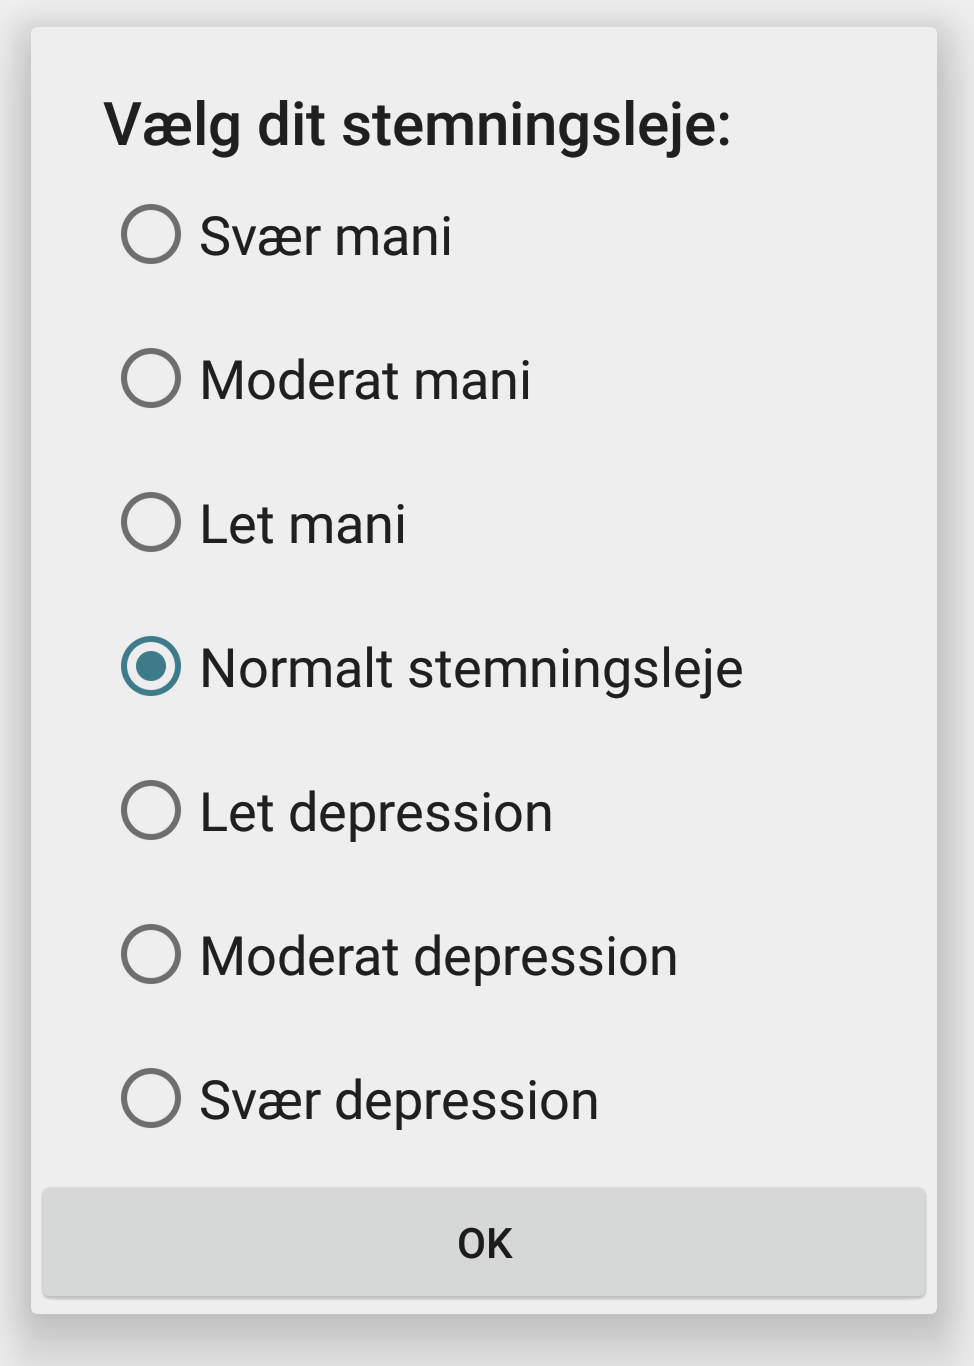
\includegraphics[width=\textwidth]{stemningsregistrering_eksempel/stemningsleje}
		\caption{Multiple choice}\label{stemreg::stemningsleje}
	\end{subfigure}
	\hfill
\begin{minipage}[b]{0.35\textwidth}
	\centering
	\begin{subfigure}[b]{\textwidth}
		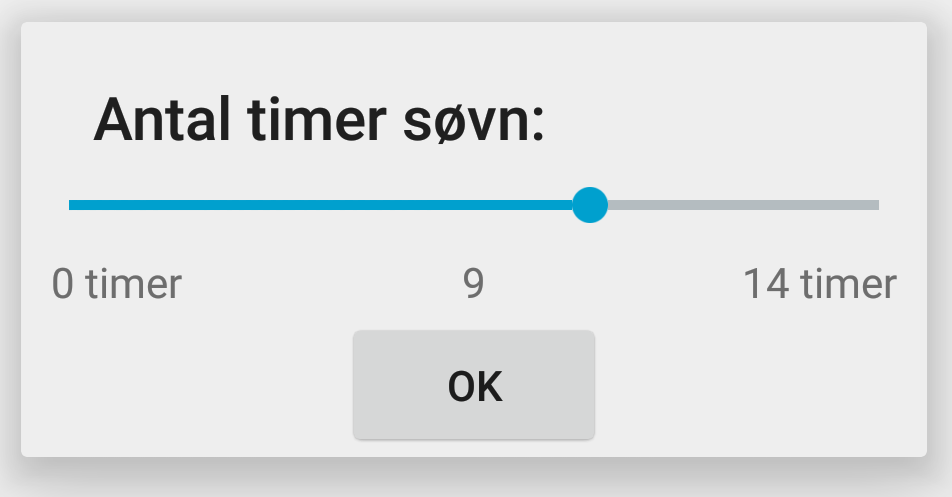
\includegraphics[width=\textwidth]{stemningsregistrering_eksempel/soevn}
		\caption{Skala}\label{stemreg::soevn}
	\end{subfigure}
	\newline 
	\begin{subfigure}[b]{\textwidth}
		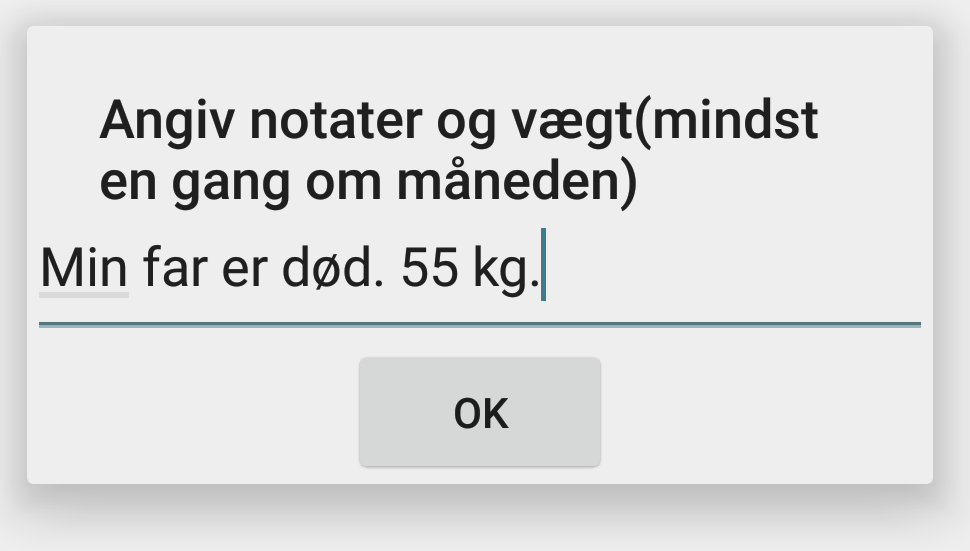
\includegraphics[width=\textwidth]{stemningsregistrering_eksempel/notater_vaegt}
		\caption{Tekst}\label{stemreg::notater_vaegt}
	\end{subfigure}	
\end{minipage}	
	\caption{Tre af de fem spørgsmål der bruges i metoden: stemningsregistrering(\cref{stemningsleje::stemningsregistrering}), for at vise de tre spørgsmåls typer.}\label{stemreg::spoergsmaal}
\end{figure}

\section{Scheduler}
For at kunne stille spørgsmål så fleksibelt som muligt er der blevet konstrueret en \textit{Scheduler}.
Stemningsregistrering og dagbog skal ske én gang om dagen, mens PANAS spørgsmål sagtens kan spredes ud over dagen for at få et bredere billede af patientens tilstand.


\paragraph{Notifikationer}
For ikke at forstyrre brugerens hverdag for meget bruger vi en notifikation til at meddele om et forestående spørgsmål.
Notifikationen indeholder spørgsmålsteksten, så patienten kan vurdere om han har tid til at besvare spørgsmålet.
Eksempler på disse notifikationer kan ses på \cref{noti}.

\begin{figure}
	\centering
	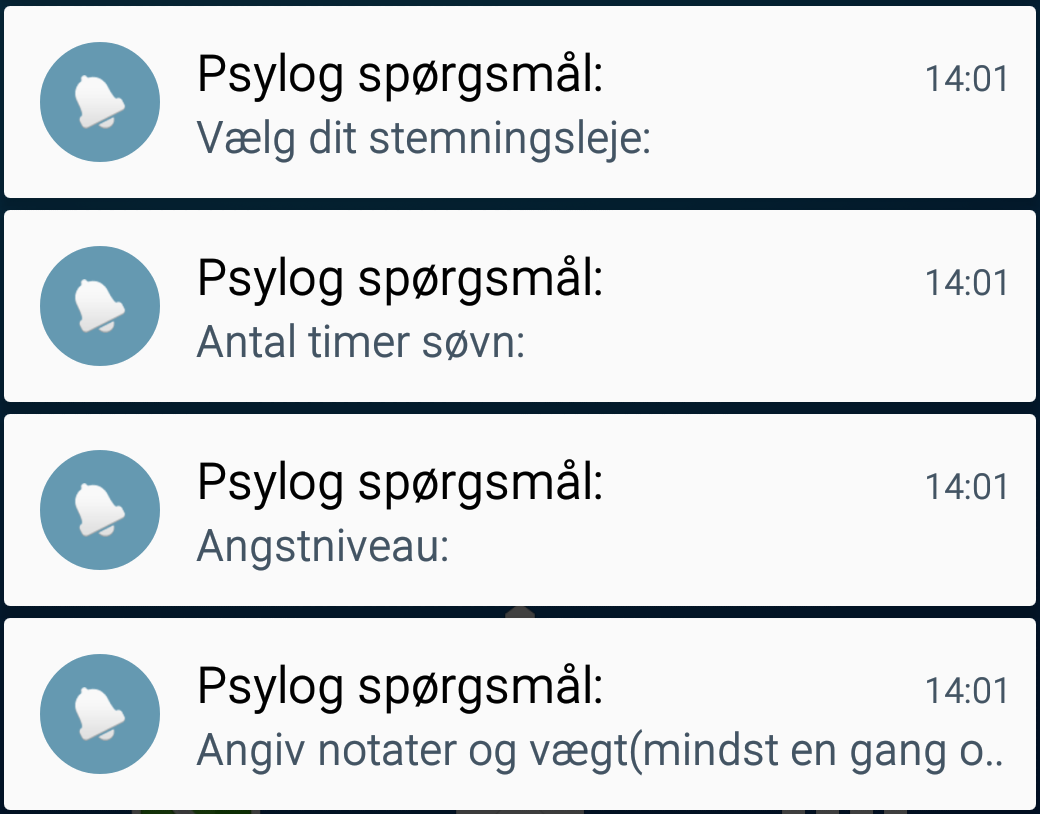
\includegraphics[width=0.4\textwidth]{stemningsregistrering_eksempel/notification_bar}
	\caption{Fire notifikationer sendt af Survey}\label{noti}
\end{figure}

Når der trykkes på notifikationen vises spørgsmålet i en dialogboks hvor patientes svar kan indføres.
Til det visuelle er der brugt standard notifikationer fra Android biblioteket \cite{android_notifications}.

For at gøre systemet endnu mere fleksibelt skal der være mulighed for at kunne udskyde et spørgsmål.
På denne måde har patienten fuld kontrol over hvornår han svarer, uden at være nødt til at skulle afbryde det han er i gang med.
Dette er endnu ikke implementeret.
